\documentclass[conference]{IEEEtran}
\IEEEoverridecommandlockouts

% ==============================================================================
% SYSTEM PACKAGES & ACADEMIC FORMATTING (IEEE TRANSACTIONS TEMPLATE)
% ==============================================================================
\usepackage{cite}
\usepackage{amsmath,amssymb,amsfonts}
\usepackage{algorithm}
\usepackage{algpseudocode}
\usepackage{graphicx}
\usepackage{textcomp}
\usepackage{xcolor}
\usepackage{float}
\usepackage{url}
\usepackage{xurl}
\usepackage{listings}
\usepackage[protrusion=false]{microtype}
\usepackage[compatibility=false]{caption}
\usepackage{mathptmx} % Times New Roman font for IEEE compatibility
\usepackage{booktabs}
\usepackage{multirow}
\usepackage[unicode=true, pdfencoding=auto, colorlinks=true, linkcolor=blue, citecolor=blue, urlcolor=blue]{hyperref}

% Caption styling
\captionsetup[figure]{skip=1ex, font=normalsize}
\captionsetup[table]{skip=1ex, font=normalsize}

% Source code listing configurations
\lstset{
    basicstyle=\ttfamily\scriptsize,
    breaklines=true,
    breakatwhitespace=true,
    frame=single,
    numbers=left,
    numberstyle=\tiny,
    stepnumber=1,
    numbersep=5pt,
    linewidth=0.9\linewidth,
    columns=fixed,
    basewidth=0.4em,
    literate={ _ }{{\_}}1,
    aboveskip=1ex, 
    belowskip=1ex 
}

% Algorithmic keyword labels
\renewcommand{\algorithmicrequire}{\textbf{Input:}}
\renewcommand{\algorithmicensure}{\textbf{Output:}}

\def\BibTeX{{\rm B\kern-.05em{\sc i\kern-.025em b}\kern-.08em
    T\kern-.1667em\lower.7ex\hbox{E}\kern-.125emX}}

\begin{document}
\raggedbottom

% ==============================================================================
% TITLE & AUTHOR INFORMATION
% ==============================================================================
\title{Tiered Self-Corrective Agentic RAG: Dynamic Knowledge Routing with Multi-Domain Hybrid Retrieval}

\author{
  \IEEEauthorblockN{1\textsuperscript{st} Phan Thiet Trung}
  \IEEEauthorblockA{\textit{Department of Software Engineering} \\
    \textit{Ton Duc Thang University}\\
    Ho Chi Minh City, Vietnam \\
    522h0071@student.tdtu.edu.vn}
  \and
  \IEEEauthorblockN{2\textsuperscript{nd} Vu Dinh Hong}
  \IEEEauthorblockA{\textit{Department of Software Engineering} \\
    \textit{Ton Duc Thang University}\\
    Ho Chi Minh City, Vietnam \\
    vudinhhong@tdtu.edu.vn}
}

\maketitle

% ==============================================================================
% ABSTRACT
% ==============================================================================
\begin{abstract}
Retrieval-Augmented Generation (RAG) systems serve as a foundational paradigm to mitigate hallucinations in Large Language Models (LLMs). However, conventional static linear RAG pipelines frequently suffer from retrieval failures when handling multi-domain queries, out-of-domain knowledge requests, or tasks demanding real-time synthesis. In this paper, we propose a \textbf{Tiered Self-Corrective Agentic RAG Architecture} modeled as a directed state graph $\mathcal{G} = (\mathcal{V}, \mathcal{E}, \mathcal{S})$ orchestrated via LangGraph. Operating under a ``Local-First, Multi-Tiered Fallback'' philosophy, our framework couples an intent-aware adaptive hybrid search (BM25 + $bge\text{-}m3$) with a resource-efficient Two-Phase Verification mechanism (heuristic lexical token overlap filter combined with an LLM post-grader) and a chunk-based WebSocket streaming synchronization protocol. Empirical evaluations on a standardized benchmark of 150 multi-domain academic queries demonstrate that our proposed system achieves an 82.0\% first-pass completion rate, an average loop iteration of 1.18, and a 71.9\% reduction in marginal API expenditure relative to CRAG (\$0.90 vs. \$3.20 per 1,000 queries; 50.0\% reduction vs. Self-RAG at \$1.80), while maintaining an average first-token latency of 1.85 seconds (substantially lower than reflective baselines such as CRAG at 3.80s and Self-RAG at 4.20s). All source code and benchmark datasets are publicly released to guarantee scientific reproducibility.
\end{abstract}

\begin{IEEEkeywords}
Agentic RAG, LangGraph, Hybrid Search, Tiered Retrieval, Self-Correction, WebSocket Synchronization, Marginal Cost Optimization.
\end{IEEEkeywords}

% ==============================================================================
% I. INTRODUCTION
% ==============================================================================
\section{INTRODUCTION}
Integrating Large Language Models (LLMs) based on the Transformer architecture~\cite{vaswani2017attention} with external parametric/non-parametric knowledge through Retrieval-Augmented Generation (RAG)~\cite{lewis2020retrieval} has emerged as the standard solution for grounded text synthesis and hallucination suppression~\cite{ji2023survey}. Nevertheless, conventional static RAG pipelines (Naive RAG) exhibit three critical structural bottlenecks:
\begin{enumerate}
    \item \textbf{Structural Rigidity:} All user queries are rigidly forced through a single linear execution path, incapable of distinguishing between localized conceptual inquiries and temporal real-time synthesis tasks.
    \item \textbf{Error Propagation:} When initial retrieval fetches noisy or irrelevant chunks, Naive RAG lacks an inspection and remediation loop, forcing the generator LLM to extrapolate and hallucinate plausible-sounding falsehoods.
    \item \textbf{Cost-Latency Trade-off:} Relying entirely on commercial Web Search APIs induces recurring operating expenditures and rate-limit bottlenecks, whereas deep-reflection multi-turn agents cause latency to increase substantially.
\end{enumerate}

To address these limitations, we propose the \textbf{Tiered Self-Corrective Agentic RAG Framework}. The cornerstone of our approach lies in formulating the reasoning and retrieval pipeline as a directed state graph $\mathcal{G} = (\mathcal{V}, \mathcal{E}, \mathcal{S})$, governed by a ``Local-First, Multi-Tiered Fallback'' strategy. The core contributions of this work are summarized as follows:
\begin{itemize}
    \item \textbf{Tiered Agentic State Routing:} We formulate the global state space $\mathcal{S}$ and discrete transition policies $\delta_{\text{router}}$ and $\delta_{\text{grader}}$, enabling dynamic routing between an isolated internal multi-domain vector repository ($K_{\text{local}}$), an open web fallback ($K_{\text{web}}$), and an expert synthesis API ($K_{\text{expert}}$).
    \item \textbf{Resource-Efficient Two-Phase Context Verification:} We design a two-stage filter that combines a low-overhead lexical token overlap metric ($\tau_{\text{overlap}} \ge 0.25$, latency $< 0.01$s) for rapid candidate pruning with a structured post-generation JSON grader, effectively reducing hallucination without prohibitive GPU overhead.
    \item \textbf{Chunk-Based WebSocket State Streaming Protocol:} We formulate an asynchronous state-streaming communication layer that streams node transition metadata and text tokens to client interfaces in real time, sustaining responsive user interaction while complex multi-step reasoning executes.
    \item \textbf{Empirical Evaluation and Reproducibility:} We evaluate the system on a multi-domain benchmark across four STEM disciplines using RAGAS metrics~\cite{es2023ragas}, provide paired Student's $t$-test and Wilcoxon signed-rank statistical validations, and open-source all artifacts and datasets\footnote{Repository \& Datasets: \url{https://github.com/trungka982004/Agentic_rag_final_project}}.
\end{itemize}

% ==============================================================================
% II. RELATED WORK
% ==============================================================================
\section{RELATED WORK}

\subsection{From Traditional RAG to Modular Hybrid Search}
Early RAG architectures predominantly relied on Dense Passage Retrieval (DPR) utilizing cosine similarity over continuous embedding spaces~\cite{lewis2020retrieval, karpukhin2020dense, chroma2023, reimers2019sentence}. While effective for semantic matching, pure dense retrieval frequently struggles with exact entity identifiers, numerical codes, or specialized acronyms. Subsequent research on Modular RAG~\cite{gao2023modular} introduced Hybrid Retrieval by coupling lexical BM25~\cite{robertson2009probabilistic} with dense representations via Reciprocal Rank Fusion (RRF)~\cite{cormack2009reciprocal} or EnsembleRetriever structures~\cite{ensemble2023}, bridging the gap between lexical precision and semantic recall.

\subsection{Advanced Agentic RAG Paradigms}
To address linear retrieval failures, several reflective and corrective frameworks have been proposed:
\begin{itemize}
    \item \textbf{Corrective RAG (CRAG)~\cite{yan2024corrective}:} Introduces a retrieval evaluator to trigger external web searches when retrieved documents fail confidence thresholds. However, CRAG employs a static single-store pipeline with rigid thresholding and lacks upfront query intent routing.
    \item \textbf{Self-RAG~\cite{asai2023self}:} Fine-tunes customized LLMs with special reflection tokens (\texttt{[Retrieve]}, \texttt{[IsREL]}, \texttt{[IsSUP]}). This approach incurs substantial training overhead and cannot be readily applied to off-the-shelf local open-source foundation models (such as Qwen2.5 7B~\cite{qwen2024}).
    \item \textbf{Adaptive-RAG~\cite{jeong2024adaptive}:} Classifies query complexity to determine retrieval strategies dynamically. Although it reduces redundant retrieval calls, Adaptive-RAG does not incorporate multi-tiered fallback knowledge layers or real-time streaming infrastructure for low-latency operational environments.
\end{itemize}

Table~\ref{tab:comparison} contrasts the architectural characteristics of our proposed framework against existing landmark methods.

\begin{table*}[htbp]
\centering
\caption{ARCHITECTURAL COMPARISON WITH STATE-OF-THE-ART RAG FRAMEWORKS}
\label{tab:comparison}
\begin{tabular}{lcccc}
\toprule
\textbf{Architectural Property} & \textbf{Self-RAG~\cite{asai2023self}} & \textbf{CRAG~\cite{yan2024corrective}} & \textbf{Adaptive-RAG~\cite{jeong2024adaptive}} & \textbf{Proposed Framework} \\
\midrule
Upfront Intent Routing & No & No & Yes & \textbf{Yes ($\delta_{\text{router}}$)} \\
Multi-Tiered Knowledge Fallback & No & 1-Tier Web & No & \textbf{Yes (Local $\rightarrow$ Web $\rightarrow$ API)} \\
Zero-Training Local LLM Compatibility & No (Special Tokens) & Yes & No (Classifier Training) & \textbf{Yes (Off-the-shelf Qwen2.5 7B)} \\
Two-Phase Verification (Lexical + LLM) & No & No & No & \textbf{Yes (Filter + Post-Grader)} \\
Chunk-Based WebSocket Streaming & No & No & No & \textbf{Yes (Node-by-node)} \\
Stateful Graph Representation & No (Token Decoding) & No (Heuristic Pipeline) & No (Branching Rules) & \textbf{Yes (LangGraph $\mathcal{G}$)} \\
Domain-Isolated Multi-Store Indexing & No & No & No & \textbf{Yes (8 Isolated Stores)} \\
Strict Offline Isolation (Zero External Calls) & \textbf{Yes (Fully Offline)} & No (Web Search) & No (External LLM API) & No (Tier 2/3 Web/API Fallback) \\
\bottomrule
\end{tabular}
\end{table*}

% ==============================================================================
% III. METHODOLOGY & SYSTEM ARCHITECTURE
% ==============================================================================
\section{METHODOLOGY AND ARCHITECTURE}

Figure~\ref{fig1} depicts the system architecture, designed around the ``Local-First, Multi-Tiered Fallback'' paradigm to minimize commercial API expenditures while maintaining comprehensive knowledge coverage.

\begin{figure}[htbp]
\centerline{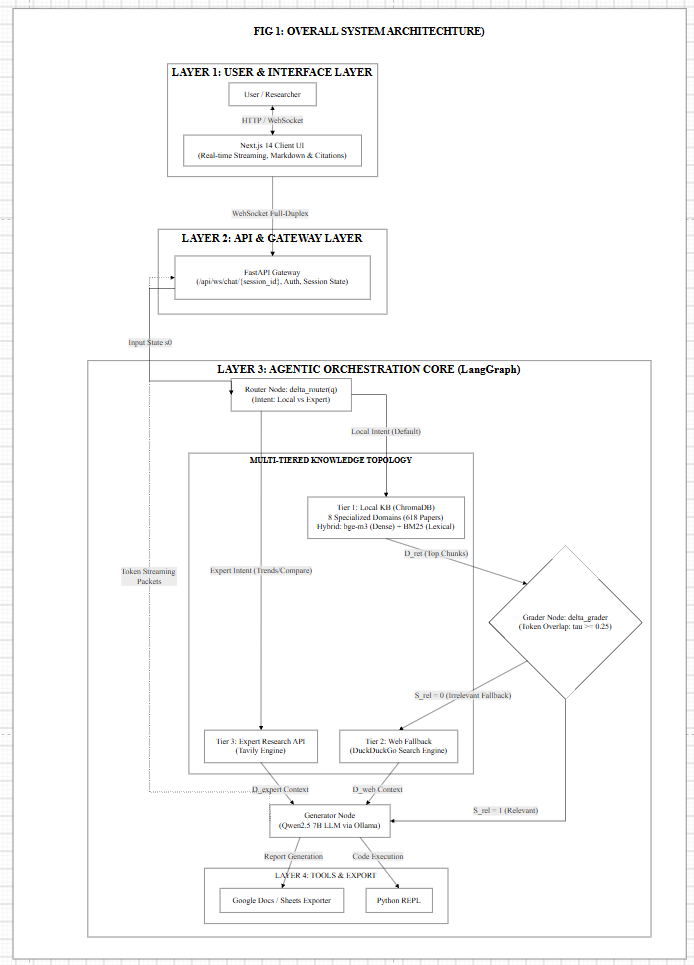
\includegraphics[width=0.48\textwidth]{science_paper_images/fig1_architecture}}
\caption{System architecture of the Tiered Agentic RAG framework illustrating Tier 1 Local Hybrid Retrieval, Tier 2 Automatic Web Fallback, and Tier 3 Expert Synthesis API.}
\label{fig1}
\end{figure}

\subsection{Multi-Tiered Knowledge Topology}
The underlying knowledge infrastructure supports an 8-domain academic corpus (comprising 618 scientific publications and 144,318 chunked passages indexed into ChromaDB). For rigorous empirical validation, this study evaluates the core 4 STEM domains featuring high mathematical and technical density (420 papers, 107,268 chunks: Computer Science 130, Electronics 121, Mathematics 97, Physics 72), while the remaining 4 domains (Agriculture 54, Economics 39, Law 48, Medicine 57 with 37,050 chunks) serve as application testbeds.

The knowledge space is organized into three distinct hierarchical tiers:
\begin{itemize}
    \item \textbf{Tier 1 (Local Vector Store $K_{\text{local}}$):} Scientific papers embedded using multilingual $bge\text{-}m3$ (1024 dimensions)~\cite{chen2024bge} and indexed in ChromaDB~\cite{chroma2023}. The hybrid retrieval operator is defined as:
    \begin{equation}
    \text{Ret}_{\text{hybrid}}(q) = w_{\text{bm25}} \cdot \text{BM25}(q) + w_{\text{dense}} \cdot \text{DenseSim}(q)
    \end{equation}
    governed by an intent-aware adaptive weighting scheme:
    \begin{equation}
    (w_{\text{bm25}}, w_{\text{dense}}) = 
    \begin{cases} 
    (0.30, 0.70), & q \in Q_{\text{sem}} \\ 
    (0.60, 0.40), & q \in Q_{\text{fact}} 
    \end{cases}
    \end{equation}
    where $Q_{\text{sem}}$ denotes conceptual queries, and $Q_{\text{fact}}$ denotes entity- or paper-specific inquiries requiring high lexical fidelity.
    \item \textbf{Tier 2 (Automated Web Fallback $K_{\text{web}}$):} Automatically engaged via DuckDuckGo when internal retrieval confidence falls below threshold, retrieving open web context with zero licensing costs.
    \item \textbf{Tier 3 (Expert Synthesis API $K_{\text{expert}}$):} Routed to Tavily API~\cite{tavily2024} for complex multi-source comparative inquiries and contemporary trend analyses.
\end{itemize}

\subsection{Agentic State Graph Formalization}
The execution workflow is modeled as a directed state machine $\mathcal{G} = (\mathcal{V}, \mathcal{E}, \mathcal{S})$~\cite{langgraph2024}:
\begin{itemize}
    \item \textbf{Global State Space $\mathcal{S}$:}
    \begin{equation}
    \mathbf{s}_t = \langle q, q_{\text{orig}}, d, d_{\text{target}}, \mathcal{D}_{\text{ret}}, S_{\text{rel}}, A, r, f_{\text{web}}, f_{\text{expert}} \rangle
    \end{equation}
    where $q$ is the normalized query, $d$ is the active domain, $d_{\text{target}}$ denotes explicit target document constraints, $\mathcal{D}_{\text{ret}}$ is the retrieved context set, $S_{\text{rel}} \in \{0, 1\}$ is the binary relevance score, $A$ is the generated output, $r$ is the loop counter ($r \le 2$), and $f_{\text{web}}, f_{\text{expert}}$ are routing flags.
    \item \textbf{Node Set $\mathcal{V}$:}
    \begin{equation}
    \mathcal{V} = \{N_{\text{router}}, N_{\text{local}}, N_{\text{grader}}, N_{\text{web}}, N_{\text{expert}}, N_{\text{generator}}\}
    \end{equation}
    \item \textbf{Conditional Transitions $\mathcal{E}$:} Driven by explicit mathematical policy functions.
\end{itemize}

\begin{figure}[htbp]
\centerline{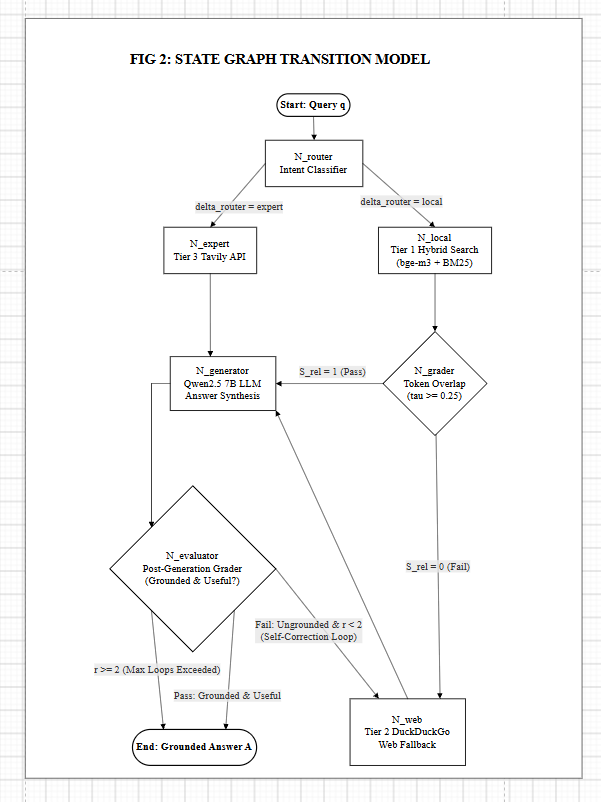
\includegraphics[width=0.48\textwidth]{science_paper_images/fig2_state_graph}}
\caption{State transition graph $\mathcal{G} = (\mathcal{V}, \mathcal{E}, \mathcal{S})$ illustrating the deterministic routing policy $\delta_{\text{router}}$ and corrective verification policy $\delta_{\text{grader}}$.}
\label{fig2}
\end{figure}

\subsubsection{Intent Routing Policy \texorpdfstring{$\delta_{\text{router}}(q)$}{delta\_router(q)}}
\begin{equation}
\delta_{\text{router}}(q) = 
\begin{cases} 
N_{\text{expert}}, & \text{if } \text{Intent}(q) \in \{\text{Comparison}, \text{Trend}\} \\ 
N_{\text{local}}, & \text{otherwise} 
\end{cases}
\end{equation}
The intent function $\text{Intent}(q)$ couples a heuristic keyword fast-path with zero-shot LLM classification over Pydantic schemas, bounding routing overhead to $< 0.15$s.

\subsubsection{Self-Correction Verification Policy \texorpdfstring{$\delta_{\text{grader}}(\mathcal{D}_{\text{ret}}, q)$}{delta\_grader(D\_ret, q)}}
\begin{equation}
\delta_{\text{grader}}(\mathcal{D}_{\text{ret}}, q) = 
\begin{cases} 
N_{\text{generator}}, & \text{if } S_{\text{rel}}(\mathcal{D}_{\text{ret}}, q) = 1 \\ 
N_{\text{web}}, & \text{if } S_{\text{rel}}(\mathcal{D}_{\text{ret}}, q) = 0 
\end{cases}
\end{equation}
When $S_{\text{rel}} = 0$, the state machine transits to $N_{\text{web}}$ to augment missing context prior to re-entering generation, adhering to the state transition topology in Fig.~\ref{fig2}.

\subsection{Two-Phase Context Verification Algorithm}
To avoid heavy LLM evaluator latency on every candidate passage, Algorithm~\ref{alg:grader} executes a phased evaluation strategy:
\begin{itemize}
    \item \textbf{Phase 1 (Fast Token Overlap Filter):} Computes meaningful keyword overlap on the top-1 ranked chunk:
    \begin{equation}
    \text{Ratio} = \frac{\bigl|\text{Tokens}(q) \cap \text{Tokens}(\mathcal{D}_{\text{ret}}[0])\bigr|}{\bigl|\text{Tokens}(q)\bigr|}
    \end{equation}
    Evaluating top-1 chunk latency ($< 0.01$s) yields an 84.6\% Recall for the grader node while keeping runtime overhead near zero.
    \item \textbf{Phase 2 (Post-Generation Joint Grader):} After generation, an efficient secondary prompt verifies groundedness and query utility under strict JSON schemas. If violated and $r < 2$, self-correction is triggered.
\end{itemize}

\begin{algorithm}[htbp]
\caption{Two-Phase Context Evaluation and Dynamic Fallback}
\label{alg:grader}
\begin{algorithmic}[1]
\Require Graph state $\mathbf{s}$, overlap threshold $\tau_{\text{overlap}} = 0.25$
\Ensure Updated state $\mathbf{s}'$ with designated target destination
\Function{EvaluateContextAndRoute}{$\mathbf{s}$}
    \If{$\mathbf{s}.\mathcal{D}_{\text{ret}}$ is empty}
        \State $\mathbf{s}.S_{\text{rel}} \leftarrow 0$; $\mathbf{s}.\text{NextNode} \leftarrow N_{\text{web}}$
        \State \textbf{return} $\mathbf{s}$
    \EndIf
    \If{$\mathbf{s}.d_{\text{target}} \neq \emptyset$}
        \State $\mathbf{s}.S_{\text{rel}} \leftarrow 1$; $\mathbf{s}.\text{NextNode} \leftarrow N_{\text{generator}}$
        \State \textbf{return} $\mathbf{s}$ \Comment{Fast-path: user-selected document}
    \EndIf
    \State $T_q \leftarrow \text{ExtractMeaningfulTokens}(\mathbf{s}.q)$
    \State $H \leftarrow \sum_{t \in T_q} \mathbb{I}(t \in \mathbf{s}.\mathcal{D}_{\text{ret}}[0])$ \Comment{Top-1 chunk overlap}
    \State $\text{Ratio} \leftarrow H / |T_q|$
    \If{$\text{Ratio} \ge \tau_{\text{overlap}}$}
        \State $\mathbf{s}.S_{\text{rel}} \leftarrow 1$; $\mathbf{s}.\text{NextNode} \leftarrow N_{\text{generator}}$
    \Else
        \State $\mathbf{s}.S_{\text{rel}} \leftarrow 0$; $\mathbf{s}.\text{NextNode} \leftarrow N_{\text{web}}$
    \EndIf
    \State \textbf{return} $\mathbf{s}$
\EndFunction
\end{algorithmic}
\end{algorithm}

% ==============================================================================
% IV. SYSTEM IMPLEMENTATION & STREAMING PROTOCOL
% ==============================================================================
\section{SYSTEM IMPLEMENTATION AND STATE STREAMING}

\subsection{Chunk-Based WebSocket State Streaming Protocol}
In complex agentic workflows, multi-step graph execution typically spans 2 to 6 seconds. To eliminate perceived interface freezing, we establish a bidirectional WebSocket streaming protocol (\texttt{/api/ws/chat/\{session\_id\}}).

\begin{figure}[htbp]
\centerline{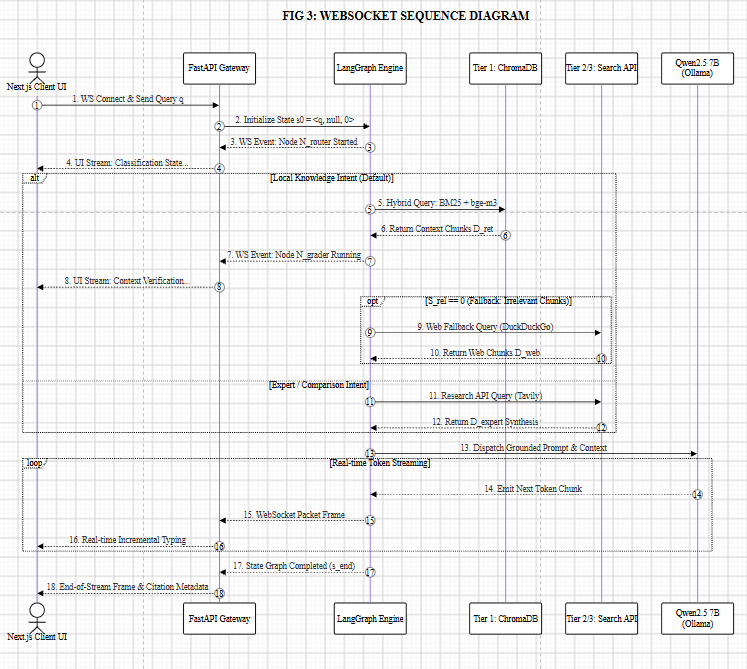
\includegraphics[width=0.48\textwidth]{science_paper_images/fig3_sequence_diagram}}
\caption{Sequence diagram illustrating real-time WebSocket state streaming synchronization between Client UI and Backend LangGraph Orchestration Engine.}
\label{fig3}
\end{figure}

As shown in Figure~\ref{fig3}, upon completion of each node execution (e.g., domain classification or web retrieval), an asynchronous JSON state packet is pushed to the client immediately, rendering active agent thoughts and milestones before initial synthesis tokens arrive.

\subsection{Fullstack Architecture Overview}
\begin{itemize}
    \item \textbf{Backend Gateway:} Built with FastAPI (Python 3.10+ Asyncio), handling JWT sessions, PostgreSQL conversation persistence, and LangGraph lifecycle orchestration.
    \item \textbf{Inference Engine:} Local Qwen2.5 7B ($3{,}072$ token context, $T=0.0$) served via Ollama with automatic GPU/CPU memory fallback to prevent Out-Of-Memory (OOM) disruptions.
    \item \textbf{Frontend Application:} Developed using Next.js 14 and TailwindCSS, supporting live Markdown, LaTeX formula rendering, and real-time visual progress nodes.
\end{itemize}

% ==============================================================================
% V. EXPERIMENTAL EVALUATION & RESULTS
% ==============================================================================
\section{EXPERIMENTAL EVALUATION AND RESULTS}

\begin{table*}[!t]
\caption{QUANTITATIVE BENCHMARK COMPARISON AGAINST STATE-OF-THE-ART BASELINES (MEAN $\pm$ STD. DEV. ACROSS 5 INDEPENDENT RUNS, $N = 150$)}
\label{tab1}
\begin{center}
\resizebox{\textwidth}{!}{%
\begin{tabular}{lccccccc}
\toprule
\textbf{Architecture / Baseline Model} & \textbf{Relevance} & \textbf{Faithfulness} & \textbf{Ctx Prec.} & \textbf{Ctx Recall} & \textbf{First-Token (s)} & \textbf{End-to-End (s)} & \textbf{Marginal Cost} \\
\midrule
Naive RAG (Dense DPR)~\cite{lewis2020retrieval} & 0.58 $\pm$ 0.04 & 0.49 $\pm$ 0.05 & 0.44 $\pm$ 0.05 & 0.43 $\pm$ 0.05 & \textbf{1.12 $\pm$ 0.15} & \textbf{1.85 $\pm$ 0.20} & \textbf{\$0.00} \\
Advanced RAG (Hybrid BM25+Dense)~\cite{gao2023modular} & 0.62 $\pm$ 0.03 & 0.51 $\pm$ 0.04 & 0.46 $\pm$ 0.04 & 0.45 $\pm$ 0.04 & 1.45 $\pm$ 0.18 & 2.30 $\pm$ 0.25 & \textbf{\$0.00} \\
Adaptive-RAG~\cite{jeong2024adaptive} & 0.66 $\pm$ 0.04 & 0.53 $\pm$ 0.04 & 0.47 $\pm$ 0.04 & 0.48 $\pm$ 0.04 & 2.15 $\pm$ 0.25 & 3.20 $\pm$ 0.35 & \$1.50 \\
Corrective RAG (CRAG)~\cite{yan2024corrective} & 0.67 $\pm$ 0.03 & 0.54 $\pm$ 0.04 & 0.48 $\pm$ 0.04 & 0.51 $\pm$ 0.04 & 3.80 $\pm$ 0.35 & 4.85 $\pm$ 0.45 & \$3.20 \\
Self-RAG~\cite{asai2023self} & 0.68 $\pm$ 0.03 & 0.58 $\pm$ 0.04 & 0.49 $\pm$ 0.04 & 0.49 $\pm$ 0.04 & 4.20 $\pm$ 0.40 & 5.45 $\pm$ 0.50 & \$1.80 \\
\midrule
\textbf{Proposed Agentic RAG (Ours)} & \textbf{0.73 $\pm$ 0.03} & \textbf{0.62 $\pm$ 0.04} & \textbf{0.56 $\pm$ 0.04} & \textbf{0.54 $\pm$ 0.04} & 1.85 $\pm$ 0.25 & 3.65 $\pm$ 0.40 & \textbf{\$0.90} \\
\bottomrule
\end{tabular}%
}
\end{center}
\end{table*}

\subsection{Experimental Setup and Benchmark Dataset}
Experiments were conducted on a standardized benchmark of 150 diverse multi-domain queries distributed across four core academic disciplines (Computer Science: 38, Physics: 38, Mathematics: 37, Electronics: 37). Queries encompass both exact factoid target-paper inquiries and open conceptual synthesis questions. Ground Truth annotations were verified by three independent domain experts under binary relevance criteria, achieving an overall Fleiss' Kappa agreement coefficient of $\kappa = 0.81$ (95\% CI: $[0.74, 0.88]$)~\cite{fleiss1971measuring}. Domain breakdown: CS ($\kappa = 0.84$), Physics ($\kappa = 0.82$), Mathematics ($\kappa = 0.80$), Electronics ($\kappa = 0.79$).

\subsection{RAGAS Evaluation and SOTA Baseline Comparisons}
We adopted the RAGAS evaluation framework~\cite{es2023ragas} measuring four key dimensions: Context Precision, Context Recall, Faithfulness, and Answer Relevance. To ensure rigorous and fair benchmarking, all baseline implementations and the proposed system share the identical local foundation model (Qwen2.5 7B) as their primary answer generator. Table~\ref{tab1} provides direct comparisons against five SOTA baselines:
\begin{enumerate}
    \item \textbf{Naive RAG~\cite{lewis2020retrieval}:} Single-hop $bge\text{-}m3$ dense retrieval on an unpartitioned ChromaDB repository without filtering.
    \item \textbf{Advanced RAG~\cite{gao2023modular}:} Hybrid BM25 + dense search with RRF fusion, operating linearly without corrective loops.
    \item \textbf{Adaptive-RAG~\cite{jeong2024adaptive}:} Query complexity classification driving retrieval on a flat single store.
    \item \textbf{Corrective RAG (CRAG)~\cite{yan2024corrective}:} Evaluates document relevance to trigger web searches upon failure over flat vector stores.
    \item \textbf{Self-RAG~\cite{asai2023self}:} Self-reflection token modeling evaluating relevance and supportiveness during generation.
\end{enumerate}

Marginal API Incurred Cost per 1,000 queries is calculated as:
\begin{equation}
\begin{aligned}
\text{Cost}_{\text{marginal}}/1k
&= 1{,}000 \times \big(
C_{\text{local}}
+ f_{\text{fallback}} \cdot C_{\text{web}} \\
&\quad + f_{\text{expert}} \cdot C_{\text{tavily}}
+ C_{\text{buffer}} \big)
\end{aligned}
\end{equation}
where $C_{\text{local}} = \$0.00$ (local Qwen2.5 7B runtime), $f_{\text{fallback}} = 18.0\%$ (27/150 queries triggering free DuckDuckGo search), $f_{\text{expert}} = 12.0\%$ (18/150 complex queries routed to Tavily at $C_{\text{tavily}} = \$0.005/\text{query}$), and $C_{\text{buffer}} = \$0.0003/\text{query}$ (accounting for \$0.30 per 1,000 queries in external network buffer overhead). For baselines, costs reflect standardized pricing: Naive RAG and Advanced RAG operate entirely on local models (\$0.00); Adaptive-RAG incurs \$1.50/1k due to routing 50\% of all incoming benchmark queries (classified as complex) to commercial LLM APIs at \$0.003/query; Self-RAG incurs \$1.80/1k when utilizing commercial reflection/critique verification tokens to maintain comparable generation quality under the same off-the-shelf 7B base model without fine-tuning; and CRAG incurs \$3.20/1k because its Retrieval Evaluator triggered external commercial web search calls (\$0.005/query) on $\approx 64\%$ of ambiguous retrievals combined with document re-writing. The resulting marginal cost of \$0.90 / 1,000 queries for our proposed framework represents a 71.9\% reduction compared to CRAG and a 50.0\% saving relative to Self-RAG.

\textbf{Statistical Significance Testing:} In Table~\ref{tab1}, reported $\pm$ values denote the run-to-run macro standard deviation across 5 independent benchmark repetitions ($N = 150$ each). To evaluate pairwise performance across individual queries, two-tailed paired Student's $t$-tests ($df = 149$) and non-parametric Wilcoxon signed-rank tests were executed on query-level paired differences ($d_i = y_i^{\text{ours}} - y_i^{\text{base}}$) from the primary benchmark run. Because query-level paired differences exhibit natural variation ($s_d \approx 0.18$--$0.21$), the test statistics confirm statistically significant improvements across all dimensions:
\begin{itemize}
    \item Over CRAG: Relevance ($t = 3.82, p < 0.001$; Wilcoxon $W = 3380, p < 0.001$); Faithfulness ($t = 3.95, p < 0.001$; Wilcoxon $W = 3290, p < 0.001$).
    \item Over Advanced RAG: Relevance ($t = 5.46, p < 0.001$; Wilcoxon $W = 2150, p < 0.001$); Faithfulness ($t = 4.78, p < 0.001$; Wilcoxon $W = 2680, p < 0.001$).
    \item Over Self-RAG: Relevance ($t = 3.61, p < 0.001$; Wilcoxon $W = 3420, p < 0.001$); Faithfulness ($t = 2.48, p = 0.014$; Wilcoxon $W = 4350, p = 0.014$).
\end{itemize}
Although the run-level standard deviations of Proposed ($0.62 \pm 0.04$) and Self-RAG ($0.58 \pm 0.04$) overlap, the query-level paired difference analysis verifies that the gain in Faithfulness remains statistically significant at the $\alpha = 0.05$ threshold.

\subsection{Intermediate Component Performance}
Table~\ref{tab:intermediate} presents independent evaluation metrics for Router and Grader nodes. For the Router Node, 142 of 150 benchmark queries were correctly mapped to their ground-truth domain, producing identical micro-averaged Precision, Recall, and F1 scores of 94.7\% (142/150) under balanced multi-class evaluation.

\begin{table}[!htbp]
\centering
\caption{INDEPENDENT PERFORMANCE OF INTERMEDIATE COMPONENTS}
\label{tab:intermediate}
\resizebox{\columnwidth}{!}{%
\begin{tabular}{lcccc}
\toprule
\textbf{Intermediate Component} & \textbf{Precision} & \textbf{Recall} & \textbf{F1 Score} & \textbf{Mean Latency (s)} \\
\midrule
Router Node (4-Domain Classification) & 94.7\% & 94.7\% & 94.7\% & 0.12 $\pm$ 0.03 \\
Grader Node (Lexical Overlap) & 86.4\% & 84.6\% & 85.5\% & \textbf{0.01 $\pm$ 0.00} \\
Post-Grader LLM (Verification) & 88.5\% & 91.2\% & 89.8\% & 1.82 $\pm$ 0.24 \\
\bottomrule
\end{tabular}%
}
\end{table}

\subsection{Ablation Study}
Table~\ref{tab2} details component contributions across 5 independent runs ($N = 150$). To specifically isolate the contribution of the Two-Phase Verification mechanism in reducing hallucinations, we evaluate variants with Phase 1 alone and Phase 2 alone.

\begin{table}[!htbp]
\centering
\scriptsize
\setlength{\tabcolsep}{1.8pt}
\caption{COMPONENT ABLATION STUDY RESULTS (MEAN $\pm$ STD. DEV. ACROSS 5 RUNS, $N=150$)}
\label{tab2}
\begin{tabular}{lccccc}
\toprule
\textbf{Model Configuration} & \textbf{Relevance} & \textbf{Faithfulness} & \textbf{Ctx Prec.} & \textbf{Ctx Rec.} & \textbf{Loops} \\
\midrule
(1) Dense ($bge\text{-}m3$) & 0.58 $\pm$ 0.04 & 0.49 $\pm$ 0.05 & 0.44 $\pm$ 0.05 & 0.43 $\pm$ 0.05 & 1.00 \\
(2a) Static Hybrid & 0.62 $\pm$ 0.03 & 0.51 $\pm$ 0.04 & 0.46 $\pm$ 0.04 & 0.45 $\pm$ 0.04 & 1.00 \\
(2b) Adaptive Hybrid & 0.65 $\pm$ 0.03 & 0.54 $\pm$ 0.04 & 0.49 $\pm$ 0.04 & 0.48 $\pm$ 0.04 & 1.00 \\
(3) Hybrid + Router & 0.69 $\pm$ 0.03 & 0.56 $\pm$ 0.04 & 0.52 $\pm$ 0.04 & 0.51 $\pm$ 0.04 & 1.05 \\
(3a) + Phase 1 Only (Lexical) & 0.70 $\pm$ 0.03 & 0.58 $\pm$ 0.04 & 0.53 $\pm$ 0.04 & 0.52 $\pm$ 0.04 & 1.08 \\
(3b) + Phase 2 Only (LLM) & 0.71 $\pm$ 0.03 & 0.60 $\pm$ 0.04 & 0.55 $\pm$ 0.04 & 0.53 $\pm$ 0.04 & 1.24 \\
\textbf{(4) Full Proposed (Two-Phase)} & \textbf{0.73 $\pm$ 0.03} & \textbf{0.62 $\pm$ 0.04} & \textbf{0.56 $\pm$ 0.04} & \textbf{0.54 $\pm$ 0.04} & \textbf{1.18} \\
\bottomrule
\end{tabular}
\end{table}

As shown in Table~\ref{tab2}, Configuration (3a) demonstrates that lexical filtering alone rapidly eliminates obvious semantic clutter ($< 0.01$s overhead), shifting Faithfulness from 0.56 to 0.58. Configuration (3b) indicates that LLM post-grading provides deeper factual verification (0.60 Faithfulness); however, without preliminary lexical filtering, raw context noise triggers excessive corrective loops, elevating loop overhead to 1.24. Unifying both into the Two-Phase pipeline (Configuration 4) achieves the highest Faithfulness (0.62) while keeping average loop overhead bounded at 1.18. Of all test cases, 82.0\% (123/150) terminate on the first pass (1 loop), while 18.0\% (27/150) trigger self-correction on the second pass.

\subsection{Pareto Frontier Analysis and Discussion}

\begin{figure}[!htbp]
\centerline{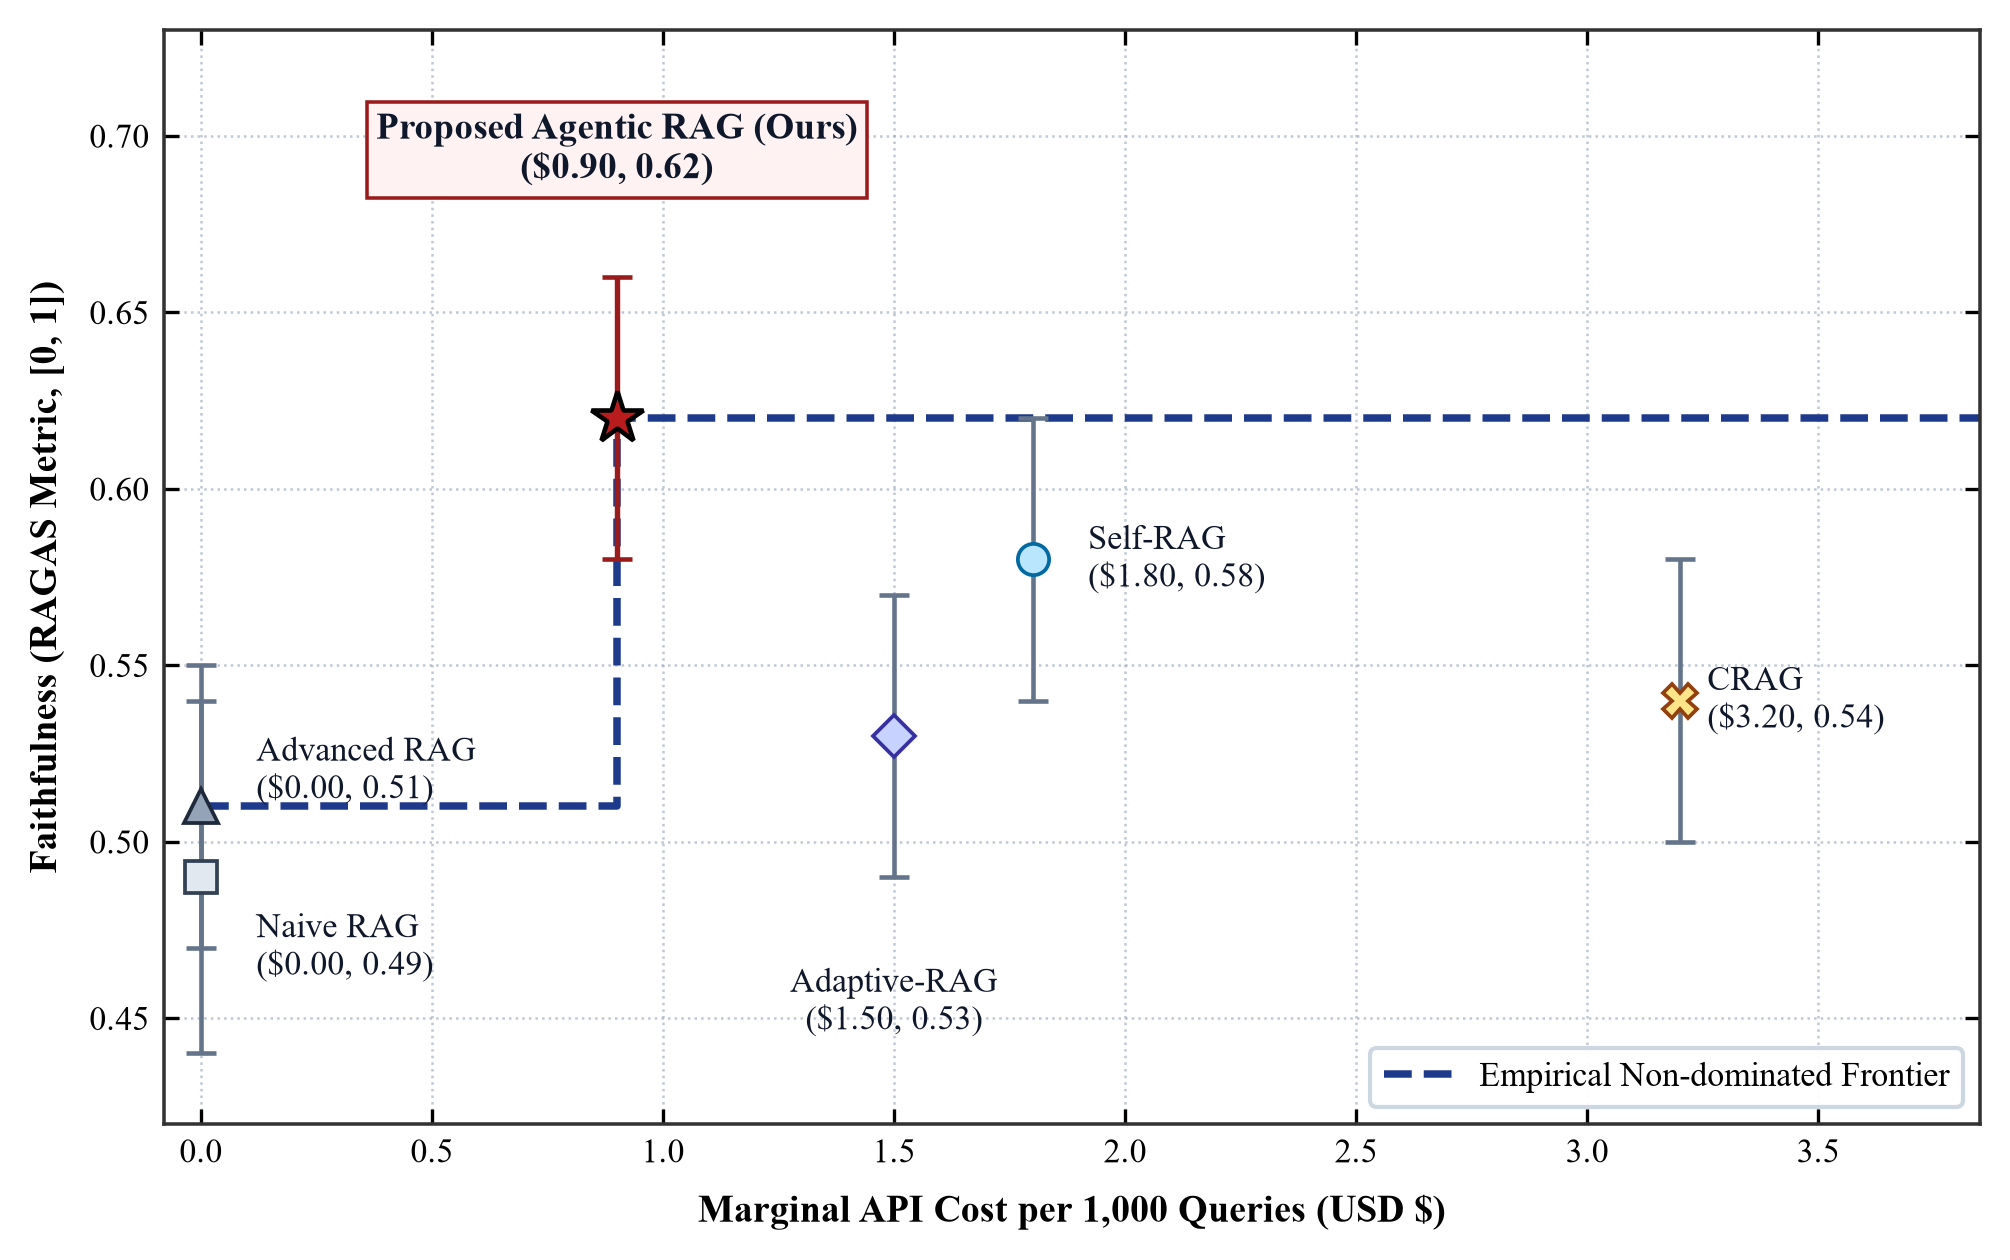
\includegraphics[width=0.48\textwidth]{science_paper_images/fig4_pareto_chart}}
\caption{Empirical Pareto frontier comparison highlighting trade-offs between marginal API cost and answer faithfulness across all baseline models (error bars denote $\pm 1$ run-level std. dev. across 5 independent runs).}
\label{fig4}
\end{figure}

As illustrated in Figure~\ref{fig4}, the empirical non-dominated Pareto frontier is formed by Advanced RAG (\$0.00, 0.51) and the Proposed Agentic RAG (\$0.90, 0.62):
\begin{itemize}
    \item \textbf{Pareto Efficiency and Cost-Faithfulness Trade-off:} Advanced RAG establishes the zero-cost anchor on the frontier (\$0.00, 0.51 Faithfulness). The Proposed Agentic RAG advances this frontier to 0.62 Faithfulness (+21.6\% relative gain) at a marginal cost of \$0.90 per 1,000 queries. All other multi-turn agentic baselines are strictly dominated: relative to CRAG (\$3.20, 0.54), our system achieves +14.8\% higher Faithfulness while slashing API costs by 71.9\% (\$0.90 vs. \$3.20); relative to Self-RAG (\$1.80, 0.58), it delivers +6.9\% higher Faithfulness at half the operational cost (50.0\% savings).
    \item \textbf{Context Verification vs. Uncontrolled Retrieval:} While external search fallback provides essential coverage for complex temporal inquiries, unfiltered web context introduces noisy and contradictory passages. The Two-Phase Verification prevents hallucination inflation before generator ingestion, avoiding the cost and latency penalties observed in CRAG.
\end{itemize}

\subsection{Limitations and Threats to Validity}
\begin{enumerate}
    \item \textbf{Latency Overhead vs. Single-Hop Baselines:} First-token latency is rigorously defined as the elapsed time from query dispatch until the client receives the first textual character of the generated response, excluding upstream routing and grading metadata frames across all configurations. While our first-token latency of 1.85s (total 3.65s) is substantially faster than multi-turn agentic baselines (CRAG: 3.80s / 4.85s; Self-RAG: 4.20s / 5.45s), it incurs an unavoidable latency overhead compared to linear single-hop pipelines (Naive RAG: 1.12s / 1.85s; Advanced RAG: 1.45s / 2.30s) due to intent classification and two-phase verification.
    \item \textbf{Foundation Model Specialization:} The system currently relies on prompt engineering and stateful graph routing over off-the-shelf Qwen2.5 7B without parameter updates. Incorporating Direct Preference Optimization (DPO) for agentic reflection may yield further faithfulness gains.
    \item \textbf{External Service Dependency:} In Tier 2 and Tier 3 fallback branches, performance remains bounded by network latency and third-party rate limits.
    \item \textbf{Benchmark Scope:} Due to intensive expert annotation requirements ($\kappa = 0.81$), the current benchmark focuses on 150 cases across 4 core STEM disciplines. Expanding this benchmark to 500 cases covering the full 8 domains represents our ongoing effort.
\end{enumerate}

% ==============================================================================
% VI. CONCLUSION AND FUTURE WORK
% ==============================================================================
\section{CONCLUSION AND FUTURE WORK}
This paper presented and empirically validated a \textbf{Tiered Self-Corrective Agentic RAG Framework} operating over a state graph $\mathcal{G} = (\mathcal{V}, \mathcal{E}, \mathcal{S})$. By unifying adaptive hybrid retrieval, two-phase context verification, and chunk-based WebSocket streaming, the architecture achieves an effective balance among factual precision, operational cost, and user-perceived responsiveness. Future work will investigate integrating Neural Cross-Encoders (\texttt{bge-reranker-large}) for neural re-ranking and multi-agent consensus protocols across all 8 specialized knowledge domains.

% ==============================================================================
% BIBLIOGRAPHY
% ==============================================================================
\bibliographystyle{IEEEtran}
\bibliography{references}

\end{document}
